% fig_dt_agreement.tex
% TR-45: DT-relay agreement breakdown pie-style horizontal bar
%
% N=1000 trials:
%   AGREE: 951 (95.10%)
%   FN (relay trips, DT flags miss): 30 (3.00%)
%   FP (DT flags trip, relay misses): 19 (1.90%)

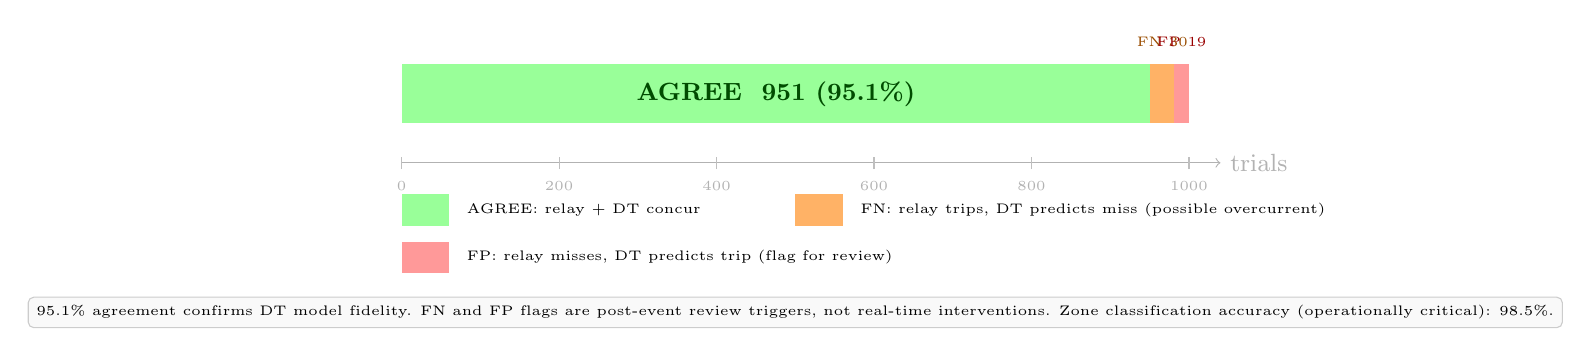
\begin{tikzpicture}[every node/.style={font=\small}]

\def\bh{0.75}
\def\btot{10.0}  %% 1000 trials → 1 cm per 100

%% AGREE: 9.51 cm
\fill[green!40]   (0.000, 0) rectangle (9.510, \bh);
\node[green!30!black, font=\small\bfseries] at (4.755, 0.375)
  {AGREE \ 951 (95.1\%)};

%% FN: 0.30 cm
\fill[orange!60]  (9.510, 0) rectangle (9.810, \bh);
\node[orange!60!black, font=\tiny, above=3pt] at (9.66, \bh)
  {FN 30};

%% FP: 0.19 cm
\fill[red!40]     (9.810, 0) rectangle (10.00, \bh);
\node[red!60!black, font=\tiny, above=3pt] at (9.905, \bh)
  {FP 19};

%% Axis
\draw[gray!60, ->] (0, -0.50) -- (10.40, -0.50) node[right] {trials};
\foreach \x/\lab in {0/0, 2/200, 4/400, 6/600, 8/800, 10/1000}{
  \draw[gray!50, thin] (\x, -0.58) -- (\x, -0.42);
  \node[gray!60, below=1pt, font=\tiny] at (\x, -0.58) {\lab};
}

%% Legend
\def\ly{-1.30}
\fill[green!40]  (0, \ly) rectangle (0.6, \ly+0.40);
\node[right=3pt, font=\tiny] at (0.6, \ly+0.20)
  {AGREE: relay + DT concur};
\fill[orange!60] (5.0, \ly) rectangle (5.6, \ly+0.40);
\node[right=3pt, font=\tiny] at (5.6, \ly+0.20)
  {FN: relay trips, DT predicts miss (possible overcurrent)};
\fill[red!40]    (0, \ly-0.60) rectangle (0.6, \ly-0.20);
\node[right=3pt, font=\tiny] at (0.6, \ly-0.40)
  {FP: relay misses, DT predicts trip (flag for review)};

%% Annotation
\node[draw=gray!40, fill=gray!5, rounded corners=2pt,
      font=\tiny, inner sep=3pt, align=center]
  at (5.0, -2.40)
  {95.1\% agreement confirms DT model fidelity.
   FN and FP flags are post-event review triggers, not real-time interventions.
   Zone classification accuracy (operationally critical): 98.5\%.};

\end{tikzpicture}
